\chapter{Einleitung}
Das Thema \ac{KI} erlangt zunehmend an Relevanz und durchdringt viele Felder.
Auch die Hochschullehre kann vom Einsatz künstlicher Intelligenzen profitieren.
Es existieren erste Versuche intelligente Systeme in die Lehre zu integrieren, wie etwa Chatbots in eingesetzten Lernmanagementsystemen, qualitative Auswertungen von Lernendendaten durch Learning Analytics und weitere \cite*[S. 18, S. 14ff.]{Witt.2020}.
\\ \\ \noindent
Abbilung \ref*{fig:entwickling_ki} veranschaulicht die Entwicklung der Verbreitung von \ac{KI} generell und in der Kategorie \glqq Studium und Lehre\grqq.
Es ist eine Tendenz dahin erkennbar, dass generell künstliche Intelligenz zunehmend vorkommt.
Zudem ist KI in der Rubrik Studium und Lehre zwar relativ betrachtet seltener vertreten, aber die Tendenz steigt.

\begin{figure}[hbtp]
    \centering
    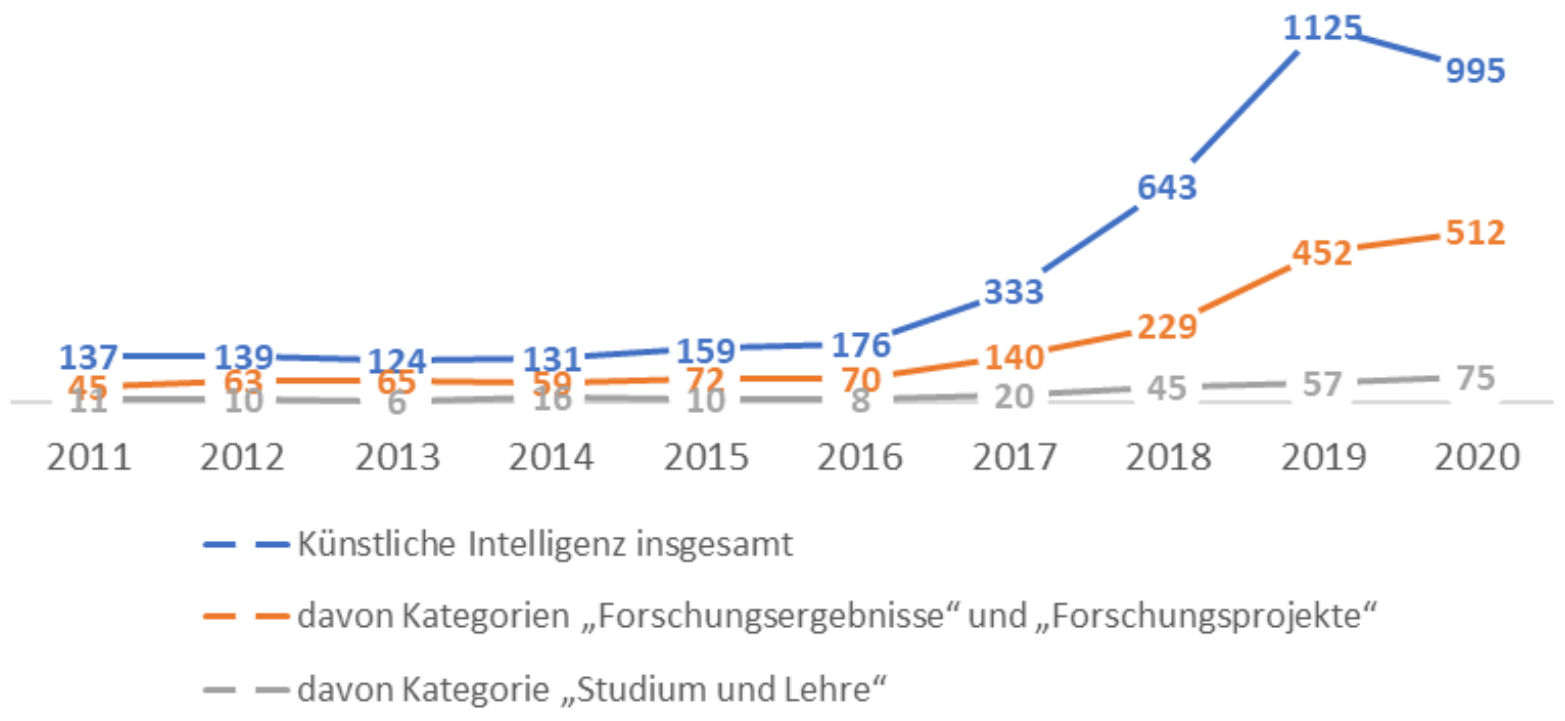
\includegraphics[width=.8\textwidth]{figures/entwicklung_historie_ki.png}
    \caption{Anzahl der Pressemitteilungen von Hochschulen und weiteren Wissenschafts-Institutionen, die das Schlagwort „Künstliche Intelligenz“ enthalten \cite*[S. 9]{Wannemacher.2021}}
    \label{fig:entwickling_ki}
\end{figure}

\noindent
Zugriffsdaten sind Daten, die beim Zugriff auf (Web-)Ressourcen erzeugt werden.
Sie können bspw. für das Reproduzieren und Beheben von Fehlern eingesetzt werden.
Es ist davon auszugehen, dass sie in Systemen in großen Mengen vorhanden sind \cite[S. 3]{Quinn.2020}.
Sie können für Analysezwecke genutzt werden, um vom Zugriffsverhalten Rückschlüsse auf andere Erkenntnisse zu erlangen.
\noindent
Für die Entwicklung von KIs sind Daten notwendig, welche für das Training einer der KI eingesetzt werden.
Hochschulen setzen in großen Teilen bereits Systeme für die Lehre ein und besitzen demnach Daten, besonders Zugriffsdaten \cite[S. 3]{Quinn.2020}.
Die zentrale Arbeitsfrage dieser Ausarbeitung ist, wie Zugriffsdaten für den Einsatz von künstlichen Intelligenzen im Kontext der Hochschullehre eingesetzt werden können.
\noindent
Hierfür wird zunächst eine Einführung in das Themenfeld KI im Kontext der Hochschullehre gegeben.
Die Paper \glqq Künstliche Intelligenz in der Hochschullehre\grqq{} von de Witt, Rampelt und Pinkwart und \glqq Another 25 Years of AIED? Challenges and Opportunities for Intelligent Educational Technologies of the Future\grqq{} von Pinkwart geben einen Überblick über aktuelle Entwicklungen über KIs in der Hochschullehre.
Hierfür werden die Erkenntnisse der Paper herausgestellt.
Anschließend folgt eine Vorstellung eines Forschungprojekts, welches mithilfe einer KI, die Zugriffsdaten des \ac{LMS} Moodle benutzt, versucht vorherzusagen, ob ein Studierender einen Kurs besteht oder durchfällt.
Im Fazit werden die Ergebnisse der Paper zusammengefast, eine Bewertung der Entwicklungen gegeben und abschließend ein Ausblick vorgeschlagen.